\section{离子化合物和共价化合物}\label{sec:2-5}

我们已经学了原子核外电子层排布的初步知识,知道元素的化学性质跟其原子的最外层电子数有密切关系。
现在,我们就可以来研究不同元素的原子是怎样形成化合物的。

\subsection{离子化合物}

% \begin{wrapfigure}[12]{r}{5cm}
%     \centering
%     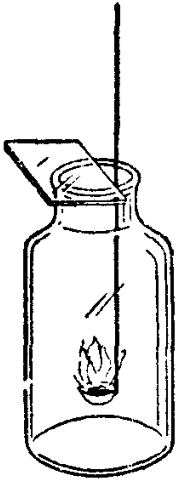
\includegraphics[width=2cm]{../pic/czhx1-ch2-13}
%     \caption{钠在氯气里燃烧}\label{fig:2-13}
% \end{wrapfigure}

我们已经知道,钠是金属元素,氯是非金属元素。
游离态的钠和氯都很容易跟别的物质发生化学反应。
它们互相起化学反应,生成化合物氯化钠(俗名食盐)。

\begin{shiyan}
    取黄豆粒大的一块钠,擦去表面的煤油,放在铺上石棉或细沙的燃烧匙里加热,
    等钠刚开始燃烧,就立刻连匙带钠伸进盛氯气的集气瓶里( 图 \ref{fig:2-13}),
    观察发生的现象。
\end{shiyan}

钠在氯气里剧烈燃烧,生成白色的氯化钠固体。

\begin{figure}[htbp]
    \centering
    \begin{minipage}[b]{7cm}
        \centering
        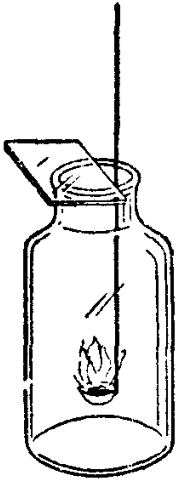
\includegraphics[width=2cm]{../pic/czhx1-ch2-13}
        \caption{钠在氯气里燃烧}\label{fig:2-13}
    \end{minipage}
    \qquad
    \begin{minipage}[b]{7cm}
        \centering
        \begin{tikzpicture}[
    >=Stealth, scale=0.6, transform shape
]
    \draw (0, 0) pic{atom={number=11}} node [above=2em] {\ce{Na}};
    \draw (6, 0) pic{atom={number=17, direction=left}} node [above=2em] {\ce{Cl}};
    \draw [->] (2.3, 0) -- (3.7, 0);

    \draw [->] (0, -1) -- (0, -2.5);
    \draw [->] (6, -1) -- (6, -2.5);

    \draw (0, -4) pic{atom={number=11, layer={2,8}}} node [above=2em] {\ce{Na+}};
    \draw (6, -4) pic{atom={number=17, layer={2,8,8}, direction=left}} node [above=2em] {\ce{Cl-}};

    \draw [->] (0, -5) -- (1.4, -6.5);
    \draw [->] (6, -5) -- (4.6, -6.5);

    \draw (2.2, -7) circle(0.5) node {\ce{Na+}}
          (3.5, -7) circle(0.8) node {\ce{Cl-}};
\end{tikzpicture}

        \caption{氯化钠的形成}\label{fig:2-14}
    \end{minipage}
\end{figure}

从钠和氯的原子结构看,钠原子的最外电子层有 1 个电子,容易失去,
氯原子的最外电子层有 7 个电子,容易得到 1 个电子,从而使最外层都达到 8 个电子的稳定结构。
所以当钠跟氯反应时,气态钠原子的最外电子层的 1 个电子转移到气态氯原子最外电子层上去,
这样,两个原子的最外电子层都成了 8 个电子的稳定结构。如图 \ref{fig:2-14} 所示。

在这个过程中,
钠原子因失去 1 个电子而带上了 1 个单位的正电荷;
氯原子因得到 1 个电子而带上了 1 个单位的负电荷。
这种带电的原子叫做\zhongdian{离子}\footnote{带电的原子团也叫离子,如硫酸根离子 \ce{SO4^{2-}},氢氧根离子 \ce{OH^-}}。
带正电的离子叫做阳离子,如钠离子(\ce{Na+});
带负电的离子叫做阴离子,如氯离子(\ce{Cl-})。
这两种带有相反电荷的离子之间有静电引力,同时两个离子的核之间以及它们的电子之间又有斥力。
当引力与斥力达到平衡时,就形成了化合物氯化钠。它不再带有电性。
\begin{fangchengshi}
    \ce{2Na + Cl2 = 2NaCl}
\end{fangchengshi}

在通常情况下,氯化钠是固体。在氯化钠固体里,
每个氯离子的周围都有 6 个钠离子,
每个钠离子的周围都有 6 个氯离子,如图 \ref{fig:2-15} 和封里彩图所示。
因此,在氯化钠固体中不存在 \ce{NaCl} 这样一个个的分子\footnote{由于
    氯化钠固体中没有一个个的 \ce{NaCl} 分子,所以,严格说来,
    \ce{NaCl} 不应叫做氯化钠的分子式,而应叫做它的 “化学式”;
    同时根据 \ce{NaCl} 计算出来的也不应叫做分子量,而应叫做 “化学式量”。
    前面所学的 \ce{Fe}、\ce{P}、\ce{C} 等,
    严格说来也不是铁、磷、碳的分子式,而是它们的化学式。
}。只有在蒸气状态时,才有 \ce{NaCl} 分子。

\begin{figure}[htbp]
    \centering
    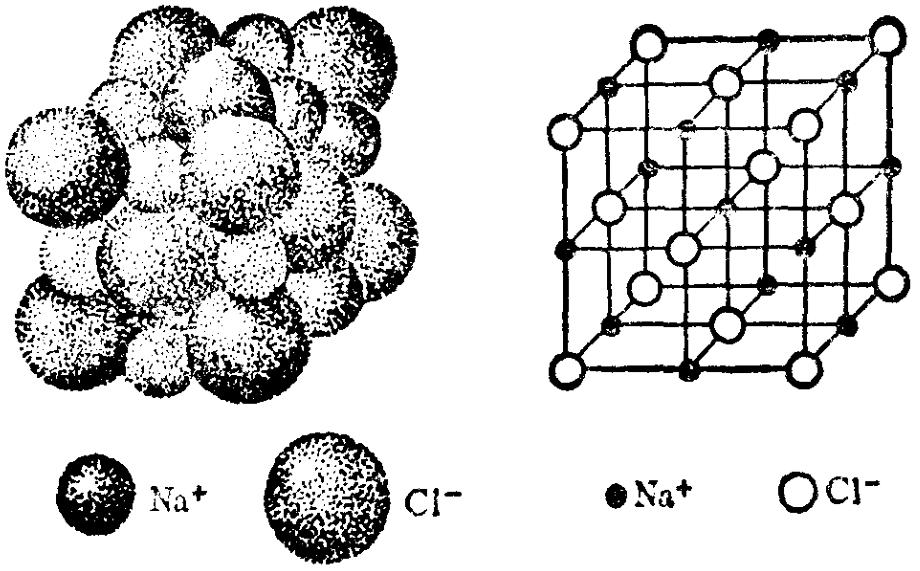
\includegraphics[width=9cm]{../pic/czhx1-ch2-15}
    \caption{氯化钠固体中的 \ce{Na+} 与 \ce{Cl-} 的排列方式示意图}\label{fig:2-15}
\end{figure}

象氯化钠这种由阴、阳离子相互作用而构成的化合物,就叫\zhongdian{离子化合物}。
如氯化钾(\ce{KCl}), 氯化镁(\ce{MgCl2}), 氯化钙(\ce{CaCl2}),
氟化钙(\ce{CaF2})等都是离子化合物。

由于在化学反应中,一般是原子的最外层电子发生变化,所以,为了简便起见,
我们可以在元素符号周围用小黑点(或 $\times$) 来表示原子的最外层电子。
这种式子叫做电子式。例如:

{
\setcharge{extra sep=3pt}
\begin{tblr}{columns={c, colsep=1em}}
    \Charge{0=\., 90=\:, 180=\:, 270=\:}{Cl}
        & \Charge{0=\.}{H}
        & \Charge{0=\., 90=\:, 180=\., 270=\:}{O}
        & \Charge{0=\.}{Na}
        & \Charge{0=\., 180=\.}{Mg}
        & \Charge{0=\., 180=\.}{Ca} \\
    氯原子 & 氢原子 & 氧原子 & 钠原子 & 镁原子 & 钙原子
\end{tblr}
}

离子化合物氯化钠和氯化钙的形成过程,可用电子式表示如下:
\begin{center}
    \schemestart
        \setcharge{extra sep=3pt}
        \chemfig{@{na}\charge{0=\chargex}{Na}}
        \+
        \chemfig{@{cl}\charge{0=\:, 90=\:, 180=\., 270=\:}{Cl}}
        \chemmove{\draw ($(na) + (0.9em, 0.3em)$) to [out=75, in=115] ($(cl) + (-0.8em, 0.3em)$);}
        \arrow(.mid east--.mid west)
        \chemfig{
            Na^+
            \chemleft[\setcharge{extra sep=3pt}\Charge{0=\:, 90=\:, 180=\chargexdot, 270=\:}{Cl}\chemright]^{-}
        }
    \schemestop\vspace*{1em}

    \schemestart
        \setcharge{extra sep=3pt}
        \chemfig{@{cl1}\charge{0=\., 90=\:, 180=\:, 270=\:}{Cl}}
        \+
        \chemfig{@{ca}\charge{0=\chargex, 180=\chargex}{Ca}}
        \+
        \chemfig{@{cl2}\charge{0=\:, 90=\:, 180=\., 270=\:}{Cl}}
        \chemmove{\draw ($(ca) + (-0.9em, 0.3em)$) to [out=115, in=75] ($(cl1) + (0.8em, 0.3em)$);}
        \chemmove{\draw ($(ca) + (0.9em, 0.3em)$) to [out=75, in=115] ($(cl2) + (-0.8em, 0.3em)$);}
        \arrow(.mid east--.mid west)
        \chemfig{
            \chemleft[\setcharge{extra sep=3pt}\Charge{0=\chargexdot, 90=\:, 180=\:, 270=\:}{Cl}\chemright]^{-}
            Ca^{2+}
            \chemleft[\setcharge{extra sep=3pt}\Charge{0=\:, 90=\:, 180=\chargexdot, 270=\:}{Cl}\chemright]^{-}
        }
    \schemestop
\end{center}


\subsection{共价化合物}

我们已经知道,氢气在氯气里燃烧,能生成氯化氢气体。
氯和氢都是非金属元素,不仅氯原子很容易获得 1 个电子形成最外层 8 个电子的稳定结构,
而且氢原子也容易获得 1 个电子形成最外层 2 个电子的稳定结构。
这两种元素的原子获得电子难易的程度相差不大,所以都未能把对方的电子夺取过来。
两种元素的原子相互作用的结果是双方各以最外层 1 个电子组成一个电子对,这个电子对为两个原子所共用,
在两个原子核外的空间运动,从而使双方最外层都达到稳定结构。
这种电子对,叫共用电子对。
共用电子对受两个核的共同吸引,使两个原子形成化合物的分子。
在氯化氢分子里,由于氯原子对电子对的吸引力比氢原子的稍强一些,所以电子对偏向氯原子一方。
因此氯原子一方略显负电性,氢原子一方略显正电性,但作为分子整体仍呈电中性。
这个过程可用电子式表示如下:
\begin{center}
    \schemestart
        \setcharge{extra sep=3pt}
        \charge{0=\chargex}{H}
        \+
        \charge{0=\:, 90=\:, 180=\., 270=\:}{Cl}
        \arrow(.mid east--.mid west)
        \setcharge{extra sep=3pt}
        H \Charge{0=\:, 90=\:, 180=\chargexdot, 270=\:}{Cl}
    \schemestop
\end{center}




象氯化氢这样以共用电子对形成分子的化合物,叫\zhongdian{共价化合物}。如水、二氧化碳等都是共价化合物。

\taolun 一百多年以前,化学家已用实验证明,任何纯净的化合物,不管它是从什么地方取来的,
或者用什么方法制取的,都有固定的组成。例如水,无论是从太平洋取来的水,还是从长江、黄河取来的水,
或者是在实验室中用人工方法制得的水,所含氢元素和氧元素的质量比都是一定的,即 $\ce{H}:\ce{O} = 1:8$。
请你用已学到的物质结构的初步知识加以解释。


\begin{xiti}

\xiaoti{用电子式表示离子化物 \ce{MgCl2} 和共价化合物 \ce{H2O} 的形成过程。}

\xiaoti{如果用下列的电子式表示氟化氢和氟化钠的形成过程:\\
    \hspace*{4em}\schemestart
        \setcharge{extra sep=3pt}
        \chemfig{@{h}\charge{0=\chargex}{H}}
        \+
        \chemfig{@{f}\charge{0=\:, 90=\:, 180=\., 270=\:}{F}}
        \chemmove{\draw ($(h) + (0.9em, 0.3em)$) to [out=75, in=115] ($(f) + (-0.8em, 0.3em)$);}
        =
        \chemfig{
            H^+
            \chemleft[\setcharge{extra sep=3pt}\Charge{0=\:, 90=\:, 180=\chargexdot, 270=\:}{F}\chemright]^{-}
        }
    \schemestop \\
    \hspace*{4em}\schemestart
        \setcharge{extra sep=3pt}
        \charge{0=\chargex}{Na}
        \+
        \charge{0=\:, 90=\:, 180=\., 270=\:}{F}
        \; =
        \setcharge{extra sep=3pt}
        Na \Charge{0=\:, 90=\:, 180=\chargexdot, 270=\:}{F}
    \schemestop \\
    你认为对吗? 说明理由。如认为不对,请加以改正。\\
    (提示:氟与氯性质相似。)
}

\xiaoti{现有一种由 $X$ 元素和 $Y$ 元素组成的离子化物,
    其分子式相当于 $X_2Y$, $X$ 离子带 1 个单位正电荷,
    两种离子的核外电子数都是 18。
}
\begin{xiaoxiaotis}

    \xxt{$X$、$Y$ 各是什么元素?画出它们的原子结构示意图。}

    \xxt{写出化合物 $X_2Y$ 的电子式。}

\end{xiaoxiaotis}

\end{xiti}

